\documentclass[aspectratio=169]{ctexbeamer} %[t]:顶端对齐
%\setlength{\parindent}{2em} % 设置缩进为2em
\usepackage{tikz}
\usetikzlibrary{arrows.meta,calc}
\usepackage{pgfplots}
\pgfplotsset{compat=1.18} %兼容到1.18版及以下版本的特性
\usepackage{amssymb,amsmath}
\usepackage{enumitem}
\usepackage{setspace} %设置行间距
\usepackage{geometry}
%\geometry{paperwidth=320mm, paperheight=180mm}
\usetheme{Madrid} %Madrid,蓝色调为主。
\usecolortheme{beaver} %beaver
\usefonttheme{professionalfonts}


\date{\today}
\begin{document}
\begin{frame}[t]{数学课程的总目标}
\begin{spacing}{1.5} %设置1.5倍行距
{\Large
通过义务教育阶段的数学学习,学生逐步:\\
\begin{enumerate}[label={\arabic*.}]
\item \textbf{会用数学的眼光观察现实世界;}\\
\item \textbf{会用数学的思维思考现实世界;}\\
\item \textbf{会用数学的语言表达现实世界。}\\
\end{enumerate}
(简称“三会”) 。\\
}
\end{spacing}
\end{frame}

\begin{frame}[t]{数学考试丢分的四大原因}
\begin{spacing}{1.5} %设置行距
{\Large
数学考试丢分的四大根本原因:\\
\begin{enumerate}[label={\arabic*.}]
\item \textbf{知识点不透彻;}\\
\item \textbf{题型不熟练;}\\
\item \textbf{计算不准确;}\\
\item \textbf{计算速度慢。} \\
\end{enumerate}
(简称“四因”) 。\\
}
\end{spacing}
\end{frame}

\begin{frame}[t]{学好数学的五个步骤}
\begin{spacing}{1.2} %设置行距
{\Large
学好数学的五个步骤:\\
\begin{enumerate}[label={\arabic*.}]
\item \textbf{发现个案(发现有趣的个案);}\\
\item \textbf{类似案例(寻找类似的案例);}\\
\item \textbf{总结规律(找到一般的规律:从特殊到一般);}\\
\item \textbf{定义证明(给出定义或证明)。} \\
\item \textbf{实际应用(应用到实践中去:从一般到特殊)。} \\
\end{enumerate}
(简称“五步骤”) 。\\
\alert{第一步到第三步:大胆假设;第四步:小心求证;第五步:放心应用。}
}
\end{spacing}
\end{frame}
% 有理数的引入
\begin{frame}{1.1 有理数的引入}
\begin{definition}
\textbf{\textcolor{orange}{正整数、0 和负整数统称为整数(integer), 正分数和负分数统称为分数(fraction).\\
整数和分数统称为有理数(rational number).}}
\end{definition}
\vspace{12pt}
\begin{columns}
\column{0.5\textwidth}
\[
\mbox{有理数}\begin{cases}
\mbox{整数} \begin{cases}
    \mbox{正整数} \\
    0 \\
    \mbox{负整数}
    \end{cases} \\
\mbox{分数}  \begin{cases}
    \mbox{正分数} \\
    \mbox{负分数}
    \end{cases}
\end{cases}
\]

\column{0.5\textwidth}
\[
\mbox{小数}\begin{cases}
\mbox{有限小数} \\
\mbox{无限小数} \begin{cases} 
\mbox{无限循环} \\
\mbox{无限不循环小数}
\end{cases}
\end{cases}
\]

%\begin{tikzpicture}
%\node (A) at(0,0) {有理数};
%\node (A1) at(2,1) {整数};
%\node (A11) at(4,2) {正整数};
%\node (A12) at(4,1) {0};
%\node (A13) at(4,0) {负整数};
%\node (A2) at(2,-1.5) {分数};
%\node (A21) at(4,-1) {正分数};
%\node (A22) at(4,-2) {负分数};
%\draw (A) -- (A1) -- (A11) (A1) -- (A12) (A1) -- (A13);
%\draw (A) -- (A2) -- (A21) (A2) -- (A22);
%\end{tikzpicture}
\end{columns}
\vspace{12pt}
\textbf{有限小数和无限循环小数是分数;\\
无限不循环小数不是分数.}
\end{frame}

% 相反数的定义及函数图象
\begin{frame}{1.2 数轴}
\begin{definition}
\textbf{\textcolor{orange}{规定了原点、正方向和单位长度的直线叫做数轴(number axis).} } \\
\end{definition}
\vspace{12pt}
\textbf{数轴的四要素:} 
\begin{enumerate}[label={\arabic*.}]
    \item \textbf{原点}
    \item \textbf{正方向}
    \item \textbf{单位长度}
    \item \textbf{直线(强调三要素的只包括前三条)}
\end{enumerate}
\vspace{12pt}
\textbf{\textcolor{blue} {数轴示例:}}
\vspace{12pt}
\begin{figure}
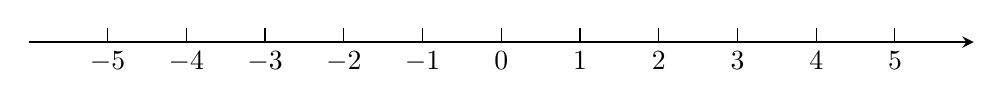
\begin{tikzpicture}
\draw [black, thick, ->, >=stealth] (-6,0) -- (6,0); 
\foreach \x in {-5, ..., 5}
	\draw (\x cm,5pt) -- (\x cm,0pt) node[anchor=north] {$\x$};
\end{tikzpicture}
\end{figure}
\end{frame}

\begin{frame}{最简数轴}
\begin{definition}
\textbf{\textcolor{orange}{规定了原点、正方向和单位长度的直线叫做数轴(number axis).} } \\
\end{definition}
\vspace{12pt}
\vspace{1cm}
\textbf{以下图形是不是一个数轴?}
\vspace{1cm}
\begin{figure}
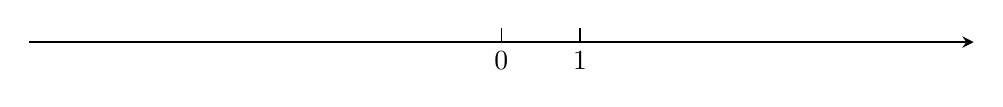
\begin{tikzpicture}
\draw [black, thick, -stealth] (-6,0) -- (6,0); 
\foreach \x in {0, 1}
 	\draw (\x cm,5pt) -- (\x cm,0pt) node[anchor=north] {$\x$};
\end{tikzpicture} 
\end{figure}
\end{frame}

\begin{frame}{类比思维}
\textbf{\textcolor{orange}{规定了原点、正方向和单位长度的直线叫做数轴(number axis).} } 
\begin{figure}
\begin{tikzpicture}

\coordinate (A) at (-5, 0);
\coordinate (B) at (-3, 0);
\coordinate (C) at (-2, 0);
\coordinate (D) at (2,0);
\coordinate (D1) at (5, 0);

\coordinate (E1) at (-5, -1);
\coordinate (F1) at (5, -1);
\coordinate (E) at (-2, -1);
\coordinate (F) at (2, -1);
\draw [Circle-Circle] (A) node [below] {A} -- node [above =0.1cm] {线段AB} (B) [below] node {B}; %画线段
%画射线
\draw [Circle-] (C) node [below] {C} -- node  [above=0.1cm] {射线CD}  (D1);
\fill (D) circle(2pt) node [below] {D}; 
 %画直线
\draw (E1)  --node  [above=0.1cm] {直线EF} (F1);
\fill (E) circle(2pt) node [below] {E}  (F) circle(2pt) node [below] {F};

\end{tikzpicture}
\end{figure}
【北京师范大学四年级上册(2013)P16】\\
\textbf{线段:线段有两个端点,线段有一定的长度。} \\
\textbf{射线:射线有一个端点,射线可以向一个方向无限延伸。} \\
\textbf{直线:直线没有端点,直线可以向两个方向无限延伸。} \\
\begin{figure}
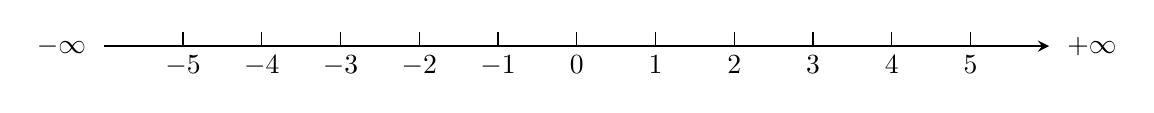
\begin{tikzpicture}
\draw [black, thick, -stealth] (-6,0) node [left=0.1cm] {$-\infty$} -- (6,0) node [right=0.1cm] {+$\infty$}; 
\foreach \x in {-5,...,5}
 	\draw (\x cm,5pt) -- (\x cm,0pt) node[anchor=north] {$\x$};
\end{tikzpicture} 
\end{figure}
\textbf{实数集$\mathbb{R}$可以用区间表示为$(-\infty, +\infty)$,$\infty$读作“无穷大”,“$-\infty$”读作“负无穷大”,“$+\infty$”读作“正无穷大”.【必修A版一册P64】}
\end{frame}
% 相反数的定义及函数图象
\begin{frame}{1.3 相反数}
\begin{definition}
\textbf{\textcolor{orange}{只有正负号不同的两个数称互为相反数(opposite number)。\\
我们规定: 0 的相反数是0 .}}
\end{definition}
\begin{columns}
\column{0.5\textwidth}
\begin{itemize}
    \item \textbf{数学表达式}:  $a + b = 0$
    \item \textbf{函数定义}:  $f(x) = -x$
    \item \textbf{定义域}: $x \in \mathbb{R}$
    \item \textbf{值域}: $y \in \mathbb{R}$
    \item \textbf{对称性}: 关于原点中心对称
\end{itemize}

\column{0.5\textwidth}
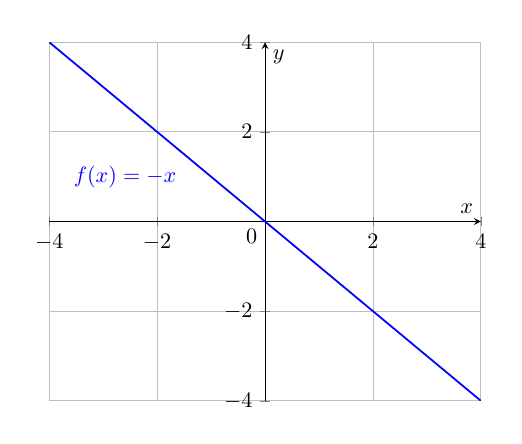
\begin{tikzpicture}[scale=0.8]
\begin{axis}[
    axis lines=middle,
    xlabel=$x$, ylabel=$y$,
    xmin=-4, xmax=4, ymin=-4, ymax=4,
    samples=500,
    grid=both,
    restrict y to domain=-4:4,
]
\addplot[blue, thick] {-x};
\node[black] at (0,0) [below left] {0};
\node[blue] at (-1.5,1) [left] {$f(x)=-x$};
\end{axis}
\end{tikzpicture}
\end{columns}
\end{frame}

% 倒数的定义及函数图象
\begin{frame}{倒数的定义及函数图象}
\begin{definition}
\textbf{\textcolor{orange}{乘积为1的两个数互为倒数。\\
注意:0没有倒数。}}
\end{definition}
\begin{columns}
\column{0.5\textwidth}
\begin{itemize}
    \item \textbf{数学表达式}:  $a \cdot b = 1$
    \item \textbf{函数定义}:  $f(x) = \dfrac{1}{x}$
    \item \textbf{定义域}: $x \in \mathbb{R}, x \neq 0$
    \item \textbf{值域}: $y \in \mathbb{R}, y \neq 0$
    \item \textbf{对称性}: 关于原点中心对称
\end{itemize}

\column{0.5\textwidth}
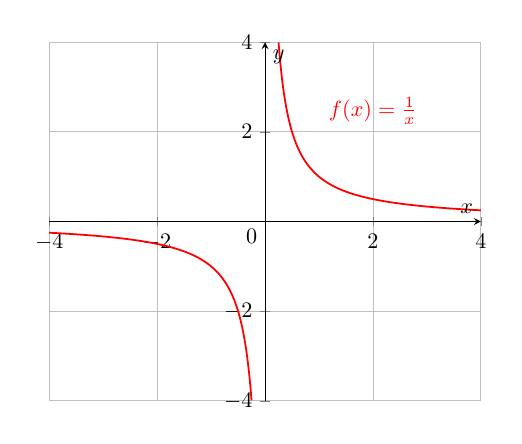
\begin{tikzpicture}[scale=0.8]
\begin{axis}[
    axis lines=middle,
    xlabel=$x$, ylabel=$y$,
    xmin=-4, xmax=4, ymin=-4, ymax=4,
    samples=500,
    grid=both,
    restrict y to domain=-4:4,
]
\addplot[red, thick] {1/x};
\node[black] at (0,0) [below left] {0};
\node[red] at (2,2) [above] {$f(x)=\frac{1}{x}$};
\end{axis}
\end{tikzpicture}
\end{columns}
\end{frame}

% 相反数与倒数的比较
\begin{frame}{相反数与倒数的比较}
\begin{columns}
\column{0.5\textwidth}
\begin{itemize}
    \item \textbf{相反数的表达式}:  $a + b = 0$
    \item \textbf{倒数的表达式}:  $a \cdot b = 1$
    \item \textbf{对称性}: 相反数与倒数均关于原点中心对称
\end{itemize}

\column{0.5\textwidth}
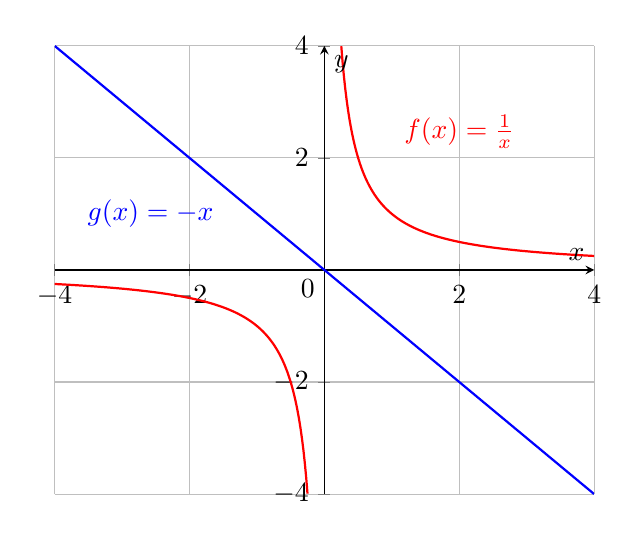
\begin{tikzpicture}[scale=1]
\begin{axis}[
    axis lines=middle,
    xlabel=$x$, ylabel=$y$,
    xmin=-4, xmax=4, ymin=-4, ymax=4,
    samples=500,
    grid=both,
    restrict y to domain=-4:4,
]
\addplot[red, thick] {1/x};
\addplot[blue, thick] {-x};
\node[black] at (0,0) [below left] {0};
\node[red] at (2,2) [above] {$f(x)=\frac{1}{x}$};
\node[blue] at (-1.5,1) [left] {$g(x)=-x$};
\end{axis}
\end{tikzpicture}
\end{columns}
\end{frame}

\begin{frame}{1.4绝对值}
\mbox{我们把在数轴上表示数$a$的点与原点的距离叫做数$a$的绝对值, 记作|$a$|.}
\begin{columns}
\column{0.45\textwidth}
\begin{enumerate}[label={\arabic*.}]
\item 一个正数的绝对值是它本身; 
\item 0 的绝对值是0;
\item 一个负数的绝对值是它的相反数.
\end{enumerate}

\begin{itemize}
    \item \textbf{数学表达式}:  $\left|  x  \right|$
    \item  \textbf{函数定义}: \[ f(x) = \begin{cases}
    x, x>0 \\
    0, x=0 \\
    -x, x<0
    \end{cases}
    \]
    \item \textbf{定义域}: $x \in \mathbb{R}$
    \item \textbf{值域}: $y \in \mathbb{R}, y \geq 0$
    \item \textbf{对称性}: 关于y轴对称
\end{itemize}

%绝对值函数图象
\column{0.5\textwidth}
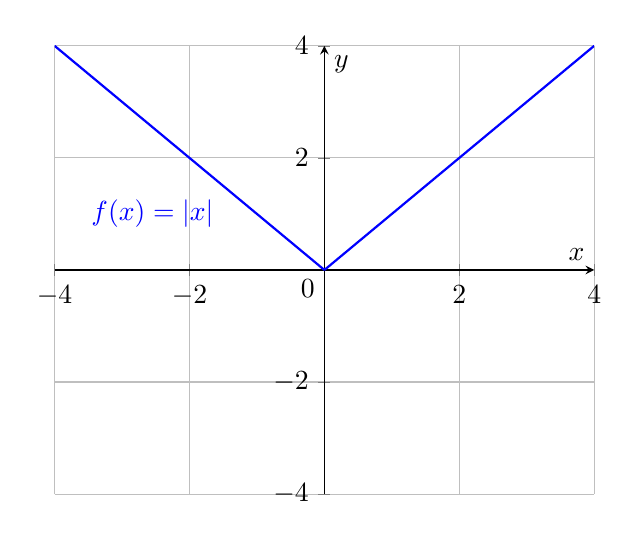
\begin{tikzpicture}[scale=1]
\begin{axis}[
    axis lines=middle,
    xlabel=$x$, ylabel=$y$,
    xmin=-4, xmax=4, ymin=-4, ymax=4,
    samples=500,
    grid=both,
    restrict y to domain=-10:10,
]
\addplot[blue, thick] {abs(x)};
\node[black] at (0,0) [below left] {0};
\node[blue] at (-1.5,1) [left] {$f(x)=|x|$};
\end{axis}
\end{tikzpicture}

\end{columns}
\end{frame}

% 绝对值与相反数的比较
\begin{frame}{绝对值与相反数的比较}
\begin{columns}

%相反数函数图象
\column{0.5\textwidth}
\textbf{相反数的函数图象}
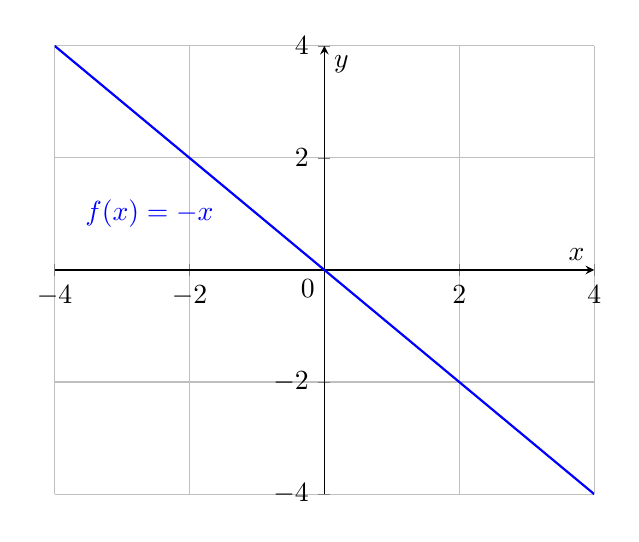
\begin{tikzpicture}[scale=1]
\begin{axis}[
    axis lines=middle,
    xlabel=$x$, ylabel=$y$,
    xmin=-4, xmax=4, ymin=-4, ymax=4,
    samples=500,
    grid=both,
    restrict y to domain=-10:10,
]
\addplot[blue, thick] {-x};
\node[black] at (0,0) [below left] {0};
\node[blue] at (-1.5,1) [left] {$f(x)=-x$};
\end{axis}
\end{tikzpicture}

%绝对值函数图象
\column{0.5\textwidth}
\textbf{绝对值的函数图象}
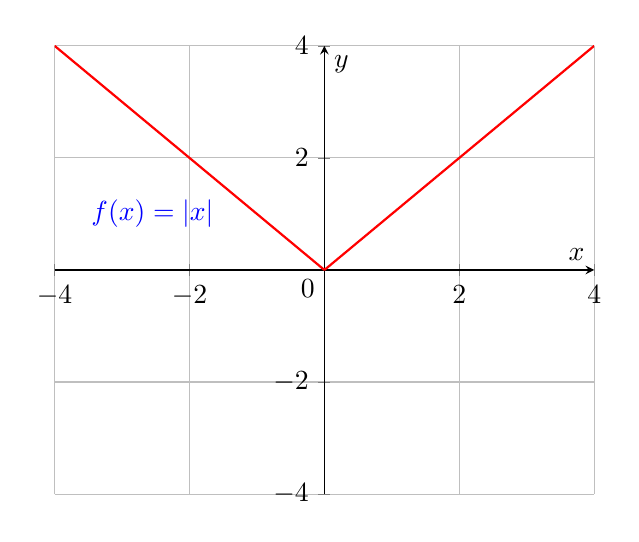
\begin{tikzpicture}[scale=1]
\begin{axis}[
    axis lines=middle,
    xlabel=$x$, ylabel=$y$,
    xmin=-4, xmax=4, ymin=-4, ymax=4,
    samples=500,
    grid=both,
    restrict y to domain=-10:10,
]
\addplot[red, thick] {abs(x)};
\node[black] at (0,0) [below left] {0};
\node[blue] at (-1.5,1) [left] {$f(x)=|x|$};
\end{axis}
\end{tikzpicture}
\end{columns}
\end{frame}


\documentclass[aspectratio=169]{ctexbeamer} %[t]:顶端对齐
\usetheme{Madrid} %Madrid,蓝色调为主。
\usecolortheme{beaver} %beaver
\usefonttheme{professionalfonts}

\usepackage{../universe}
\uBigPaper

\date{\today}
\begin{document}

% 1.5 有理数的代销比较
\begin{frame}{1.5有理数的大小比较规则}
\begin{block}{有理数大小比较法则}
\begin{enumerate}[label={\arabic*.}]
  \item 数轴上右边的数比左边的数\alert{大}
  \item 正数 \alert{>} 0
  \item 负数 \alert{<} 0
  \item 正数 \alert{>} 负数
  \item 两个负数比较,绝对值大的反而\alert{小}!
\end{enumerate}
\end{block}

\end{frame}

\begin{frame}{数轴比较法}
\begin{example}
  把下列各数表示在数轴上,并用"<"连接:\\
  $-2,\ 0,\ 3,\ -3.5,\ 1.5$
\end{example}

\pause
\begin{block}{解:}
\begin{enumerate}[label={\arabic*.}]
  \item 画数轴并标出所有数
  \begin{figure}
  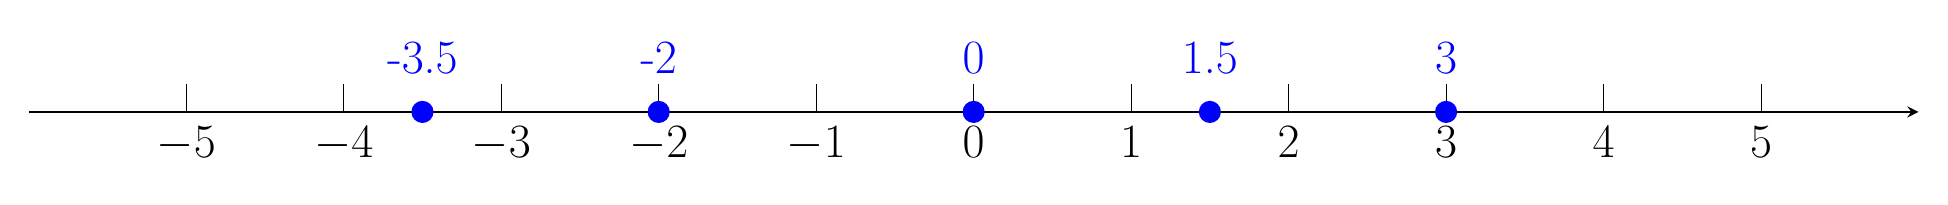
\begin{tikzpicture}[scale=2]
  \fontsize{16}{20}\selectfont
  \draw [black, thick, ->, >=stealth] (-6,0) -- (6,0); 
  \foreach \x in {-5, ..., 5}
  	\draw (\x cm,5pt) -- (\x cm,0pt) node[anchor=north] {$\x$};
  \foreach \x in {-2, 0, 3, -3.5, 1.5}
    \fill [blue] (\x,0) circle(2pt) node [above=0.3cm] {\x};
  \end{tikzpicture}
  \end{figure}
  \item 从左到右(从小到大)排列
  \item 结果:$-3.5 \alert{<} -2 \alert{<}  0 \alert{<}  1.5 \alert{<}  3$
\end{enumerate}
\end{block}
\end{frame}

\begin{frame}{两负数的绝对值比较法}
\textbf{两个负数比较,绝对值大的反而\alert{小}!}
\begin{example}
(1) -3 与 -5 哪个大? (2) -1.3 与 -3 哪个大?\\
\end{example}
\pause
\begin{block}{解:}
(1) \\
$| -3 | = 3, \quad | -5 | = 5, $ \\
$\because 3 < 5, $ \\
$\therefore -3 > -5$ \\
(2) \\
$| -1.3 | = 1.3, \quad |-3| = 3, $ \\
$\because 1.3 < 4, $\\
$\therefore -1.3 > -3$
\end{block}
\end{frame}

\end{document}
\documentclass[aspectratio=169]{ctexbeamer} %[t]:顶端对齐
\usetheme{Madrid} %Madrid,蓝色调为主。
\usecolortheme{beaver} %beaver
\usefonttheme{professionalfonts}

\usepackage{universe}
\uBigPaper

\date{\today}
\begin{document}

\begin{frame}[t]{1.6 有理数的加法法则}
\begin{spacing}{1.1} %设置行距
\normalsize
\begin{enumerate}[label={\arabic*.}]
\item 同号两数相加, 取与加数相同的正负号, 并把绝对值相加; \\
$\text{当}a,b  > 0\text{时,}$ \\
$(+a) + (+b) = +(a+b) = a + b$ \\
$(-a) + (-b) = -(a+b)$ \\
\item 绝对值不相等的异号两数相加, 取绝对值较大的加数的正负号, 并用较大的绝对值减去较小的绝对值; \\
$\text{当}a > b > 0\text{时,}$ \\
$(-a) + (+b) = -(a-b)$ \\
$(+a) + (-b) = +(a-b) = a - b$ \\
\item 互为相反数的两个数相加得0; \\
 $a + (-a) = 0$ \\
\item 一个数与0 相加, 仍得这个数. \\
$a + 0 = 0 $\\
\end{enumerate}
\end{spacing}
\end{frame}

\begin{frame}[t]{有理数加法的运算律}
\begin{spacing}{1.5} %设置行距
\Large
\begin{enumerate}[label={\arabic*.}]
\item 加法交换律:两个数相加,交换加数的位置,和不变. \\
$a + b = b + a$
\item 加法结合律: 三个数相加, 先把前两个数相加,或者先把后两个数相加,和不变. \\
$(a + b) + c = a + (b + c)$
\end{enumerate}
\end{spacing}
\end{frame}

\begin{frame}[t]{有理数去括号规则}
\begin{spacing}{1.2} %设置行距
\Large
括号前的符号与数字前的符号存在下列关系,则:
\begin{enumerate}[label={\arabic*.}]
\item 同号取正(去括号,取正号) \\
$+(+a) = +a = a$ \\
$-(-a) = +a = a$ 
\item 异号取负(去括号,取负号)\\
$-(+a) = -a$ \\
$+(-a) = -a$ \\
\end{enumerate}
\end{spacing}
\end{frame}

\end{document}
\documentclass[aspectratio=169]{ctexbeamer} %[t]:顶端对齐
\usetheme{Madrid} %Madrid,蓝色调为主。
\usecolortheme{beaver} %beaver
\usefonttheme{professionalfonts}

\usepackage{universe}
\uBigPaper

\date{\today}
\begin{document}

\begin{frame}[t]{1.7 有理数的减法}
\begin{spacing}{1.5}
\Large
有理数的减法法则:\\
\begin{enumerate}[label={\arabic*.}]
\item 减去一个数, 等于加上这个数的相反数.\\
$ a - b = a + (-b)$ \\
$ a - (-b) = a + (+b) = a + b$ \\
\end{enumerate}
\end{spacing}
\end{frame}

\end{document}
\begin{frame}[t]{1.8 有理数的加减混合运算}
\begin{spacing}{1.5}
\hspace*{2em} 算式(- 8) - (- 10) + (- 6) - (+ 4) 是有理数的加减混合运算, 可以按照运算顺序, 从左到右逐步计算; 也可以应用有理数的减法法则, 把它改写成( - 8) + (+ 10) + (- 6) + (- 4), 统一为只有加法运算的和式.\\
\hspace{2em} 在一个和式里, 通常把各个加数的括号和它们前面的加号省略不写. 如上式可写成省略加号的和的形式:\\
\[- 8 + 10 - 6 - 4.\] \\
\hspace*{2em} 这个式子仍可看作和式, 读作“负8、正10、负6、负4 的和”. 从运算意义看, 上式也可读作“负8 加10 减6减4”.
\end{spacing}
\end{frame}


\begin{frame}[t]{加法运算律在加减混合运算中的应用}
\begin{spacing}{1.5}
\hspace{2em} 因为有理数的加减法可以统一成加法, 所以在进行有理数的加减混合运算时, 可以适当应用加法运算律, 简化计算.\\
例2 计算: \\
(1) - 24 + 3.2 - 16 - 3.5 + 0.3; \\
(2) $0 - 21\dfrac{2}{3} + \left(+3\dfrac{1}{4}\right) - \left(-\dfrac{2}{3} \right) - \left(+\dfrac{1}{4} \right)$ . 
\end{spacing}
\end{frame}

\begin{frame}[t]{加法运算律在加减混合运算中的应用}
\begin{spacing}{1.4}
解:\\
(1) - 24 + 3.2 - 16 - 3.5 + 0.3 \\
= -24 - 16 -3.5 + 3.2 + 0.3 \\
= -40 - 3.5 + 3.5 \\
= -40. \\
(2) $0 - 21\dfrac{2}{3} + \left(3\dfrac{1}{4}\right) - \left(-\dfrac{2}{3} \right) - \left(+\dfrac{1}{4} \right)$  \\
$= - 21\dfrac{2}{3} + \left(3\dfrac{1}{4}\right) + \left(\dfrac{2}{3} \right) - \left(\dfrac{1}{4} \right)$ \\
$= - 21\dfrac{2}{3} + \left(\dfrac{2}{3} \right) + \left(3\dfrac{1}{4}\right) - \left(\dfrac{1}{4} \right)$ \\
$= -21 + 3 $\\
$= -18.$
\end{spacing}
\end{frame}
\end{document}